\section{Hardware cache coherence}
    \begin{tcolorbox}[violet]
        A small reminder before starting: a cache contains usually the state (valid/invalid), the tag array and the data array that keeps cache blocks (a cache block == a cache line). \\
        \textbf{4Cs cache miss model:}
        \begin{itemize}[left=10pt, label=\textbullet]
            \item Compulsory: access data for the first time.
            \item Capacity: when the cache is not big enough.
            \item Conflict: when two addresses map to the same set and way of the cache evicting one of them. 
            \item Coherence: when a block is removed due to coherence messages from another core.
        \end{itemize}
    \end{tcolorbox}
    Due to sharing data, incoherence appears between different caches. More specifically, when you're updating a value and reading a different copy. There is different ways to assure coherence we'll see two of them with their protocol.\\
\subsection{Bus-based systems}
    In bus-based systems, we have to add independent ``cache controllers'' to each core where each controller: is a FSM, sees all remote processor actions, takes coherence actions depending on block's state and protocol.
    \begin{tcolorbox}[rouge]
         \textbf{MESI protocol:} \important{M}odified, \important{E}xclusive, \important{S}hared and \important{I}nvalid states.
        \begin{itemize}[left=10pt, label=\textbullet]
            \item Modified: this cache has updated the value and holds the authoritative copy. 
            \item Exclusive: this cache has an exclusive copy. 
            \item Shared: one or more caches hold the value. 
            \item Invalid.
        \end{itemize}
        Core actions:
        \begin{itemize}[left=10pt, label=\textbullet]
            \item PRd: processor attempts to read a line.
            \item PWr: processor attempts to write a line.
        \end{itemize}
        Remote actions:
        \begin{itemize}[left=10pt, label=\textbullet]
            \item BusRd: obtain copy of a line with no intent to modify. 
            \item BusRdX: obtain copy of a line with intent to modify.
            \item BusInv: get rid of other copies.
            \item DataWB: put updated value of a line on the bus.
        \end{itemize}
    \end{tcolorbox}
    \newpage
    \textbf{MESI protocol state diagram:}
    \begin{center}
    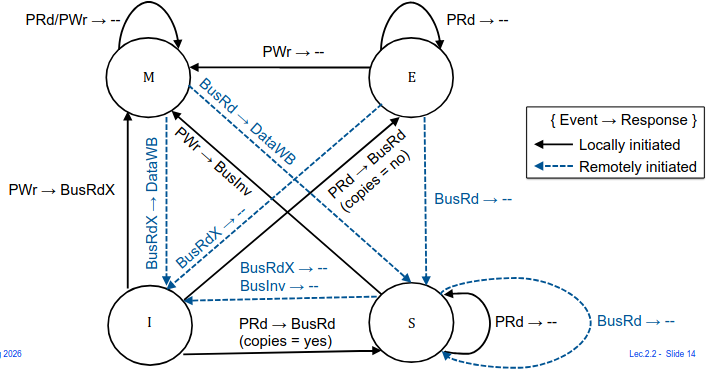
\includegraphics[width=9cm]{images/9.png}
    \end{center}
    Example:
    \begin{center}
    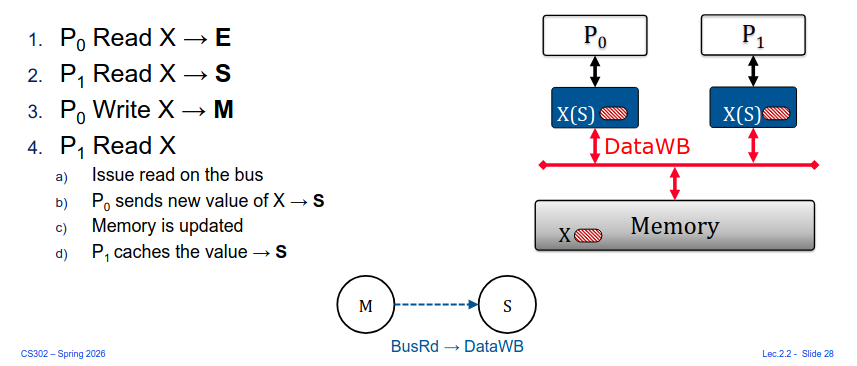
\includegraphics[width=9cm]{images/10.png}
    \end{center}
    The main problem with bus-based systems is that the bus becomes a bottleneck: as the number of cores increases, the traffic on the bus grows, leading to contention and reduced performance. That's why we'll introduce the point-to-point network organization.
\subsection{Point-to-point systems}
In the point-to-point system, the message is more scalable and have an explicit source and destination. For example, Intel Skylake uses a ring:
    \begin{center}
    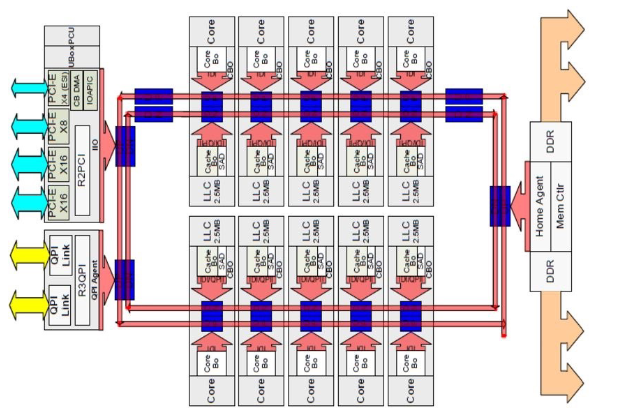
\includegraphics[width=9cm]{images/11.png}
    \end{center}
    \begin{remark}{Remark}
        In a ring (point-to-point) network, messages travel only along the path between sender and receiver, so links not on the path remain free, reducing overall traffic compared to a shared bus.   
    \end{remark}
    Now each core no longer sees all of the messages, so we need to add another protocol controller to the MESI protocol into the system.\\
    \newpage
    \textbf{Directory-based protocol:}
    \begin{tcolorbox}[vert]
        In the directory-based protocol, we use a \important{coherence directory}. The directory tracks all caches that contain a particular block, then all messages leaving the core are first sent to the directory and it takes the appropriate actions, and respond to the original cache request. The directory serves as a per-block address or
    \end{tcolorbox}
    \begin{tcolorbox}[rouge]
        Cache to directory messages: 
        \begin{itemize}[left=10pt, label=\textbullet]
            \item GetRd: get copy to read, 
            \item GetWr: get copy to modify, 
            \item UpGrd: get rid of other copies, 
            \item DataWB: write back a line, 
            \item Ack: acknowledge message.
        \end{itemize}
        Directory to cache messages:
        \begin{itemize}[left=10pt, label=\textbullet]
            \item DwnGrd: go from E/M \textrightarrow S, 
            \item Inv: get rid of your copy, 
            \item Fill: here is a copy of the line,
            \item Ack: acknowledge message.
        \end{itemize}
    \end{tcolorbox}\\
    Example:
    \begin{center}
    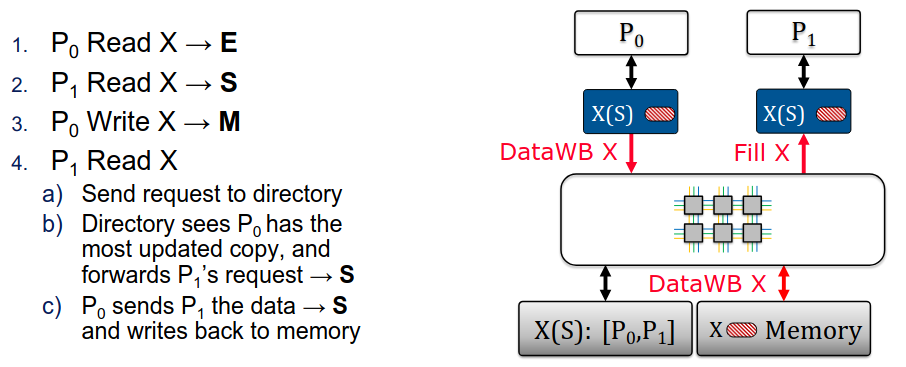
\includegraphics[width=9cm]{images/12.png}
    \end{center}
    \begin{tcolorbox}[vert]
        The \important{directory entry} contain: 2 bits storing the MESI coherence state, 39 bits containing the cache tag and $\log_2\left(\text{Cores}\right)$ bits identifying the core associated with this entry.
    \end{tcolorbox}
    The size of directory is dependent of the number and the size of caches. If there is two processor with 4-ways associative caches, then the directory must be 8-way associative:
    \begin{center}
    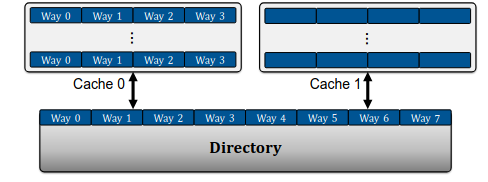
\includegraphics[width=9cm]{images/13.png}
    \end{center}
    But centralized directory can also be a source of contention, so we can distribute the directory across L2 cache banks, with each memory block having a home bank that tracks which L1 caches hold copies.
    \newpage
    \textbf{Access to the directory:}\\
    \begin{tcolorbox}[vert]
        If we do the structure that we saw before for the directory, for four cores with 4-way caches, we need to have a 16-way associative cache! This is bad for latency and power. To allow this is the \important{sparse directory}, we can split the cache and take more tag bits to index.
    \end{tcolorbox}
    \begin{center}
    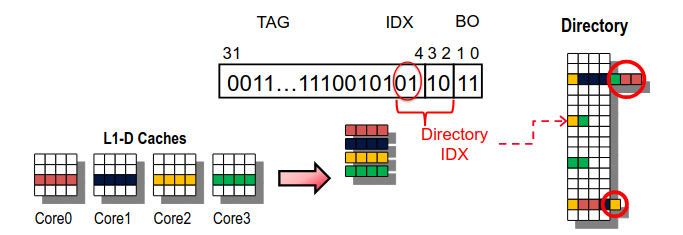
\includegraphics[width=9cm]{images/14.png}
    \end{center}
    Now the problem is that we can have conflict easily! The solution is to make a bigger directory and use more tag bits to index.
    \begin{image}{With this structure, we'll have low conflict rate, but a large area overhead\ldots}
        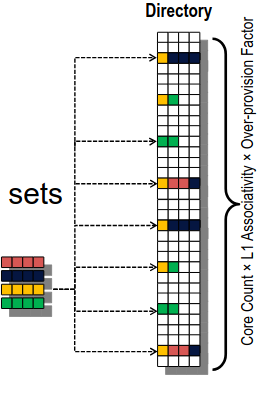
\includegraphics[width=3.5cm]{images/15.png}
    \end{image}
